\chapter{M\'odulos de Inventario y Proveedores}

\section{Inventario}

El m\'odulo de inventario gestiona productos y servicios ofrecidos por la
cl\'{\i}nica. Los productos pueden ser de cuatro tipos:

\begin{longtable}{|l|l|}
\hline
\textbf{Tipo} & \textbf{Descripci\'on} \\
\hline
medication & Medicamentos y f\'armacos \\
supply & Insumos y materiales \\
food & Alimentos y dietas \\
service & Servicios veterinarios \\
\hline
\end{longtable}

\subsection{Server Actions}

El archivo \texttt{lib/actions/products.ts} implementa CRUD completo con
tipado de interfaz:

\begin{lstlisting}[style=typescript, caption=Interfaz ProductInput]
export interface ProductInput {
  name: string;
  description: string;
  type: string;
  sku: string;
  price: string;
  costPrice: string;
  stockQuantity: number;
  reorderPoint: number;
}
\end{lstlisting}

\subsection{Alerta de Reorden}

El sistema alerta visualmente cuando el stock de un producto est\'a por
debajo del punto de reorden (\texttt{reorderPoint}), permitiendo a la
cl\'{\i}nica identificar r\'apidamente productos que necesitan
reabastecimiento.

\subsection{Server Actions}

\begin{lstlisting}[style=typescript, caption=Productos - Patron CRUD estandar]
export async function getProducts() {
  const clinicId = await getCurrentClinicId();
  return db
    .select()
    .from(schema.products)
    .where(eq(schema.products.clinicId, clinicId))
    .orderBy(schema.products.name);
}

export async function createProduct(data: ProductInput) {
  const clinicId = await getCurrentClinicId();
  await db.insert(schema.products).values({
    clinicId,
    name: data.name,
    description: data.description || null,
    type: data.type as any,
    sku: data.sku || null,
    price: data.price,
    costPrice: data.costPrice || null,
    stockQuantity: data.stockQuantity,
    reorderPoint: data.reorderPoint || null,
  });
  revalidatePath('/inventory');
}
\end{lstlisting}

\section{Proveedores}

El m\'odulo de proveedores gestiona las empresas que suministran productos
a la cl\'{\i}nica.

\subsection{Server Actions}

\begin{lstlisting}[style=typescript, caption=Proveedores - Patron CRUD estandar]
export async function getSuppliers() {
  const clinicId = await getCurrentClinicId();
  return db
    .select()
    .from(schema.suppliers)
    .where(eq(schema.suppliers.clinicId, clinicId))
    .orderBy(schema.suppliers.name);
}

export async function createSupplier(data: SupplierInput) {
  const clinicId = await getCurrentClinicId();
  await db.insert(schema.suppliers).values({
    clinicId,
    name: data.name,
    contact: data.contact || null,
    email: data.email || null,
    phone: data.phone || null,
    address: data.address || null,
  });
  revalidatePath('/suppliers');
}
\end{lstlisting}

\section{P\'aginas}

\subsection{Inventario (/inventory)}

\begin{itemize}[leftmargin=*]
    \item Tabla responsiva con nombre, tipo, SKU, precio, stock.
    \item Alerta visual (fondo rojo/amarillo) cuando stock $<$ reorderPoint.
    \item Acciones: editar, ver detalle.
\end{itemize}

\subsection{Proveedores (/suppliers)}

\begin{itemize}[leftmargin=*]
    \item Vista en tarjetas con grid responsivo.
    \item Cada tarjeta muestra logo/nombre, contacto, email, tel\'efono.
    \item Acciones: editar.
\end{itemize}

Ambos m\'odulos siguen el mismo patr\'on de implementaci\'on: CRUD con
revalidaci\'on de ruta y filtrado por cl\'{\i}nica.

\begin{figure}[H]
    \centering
    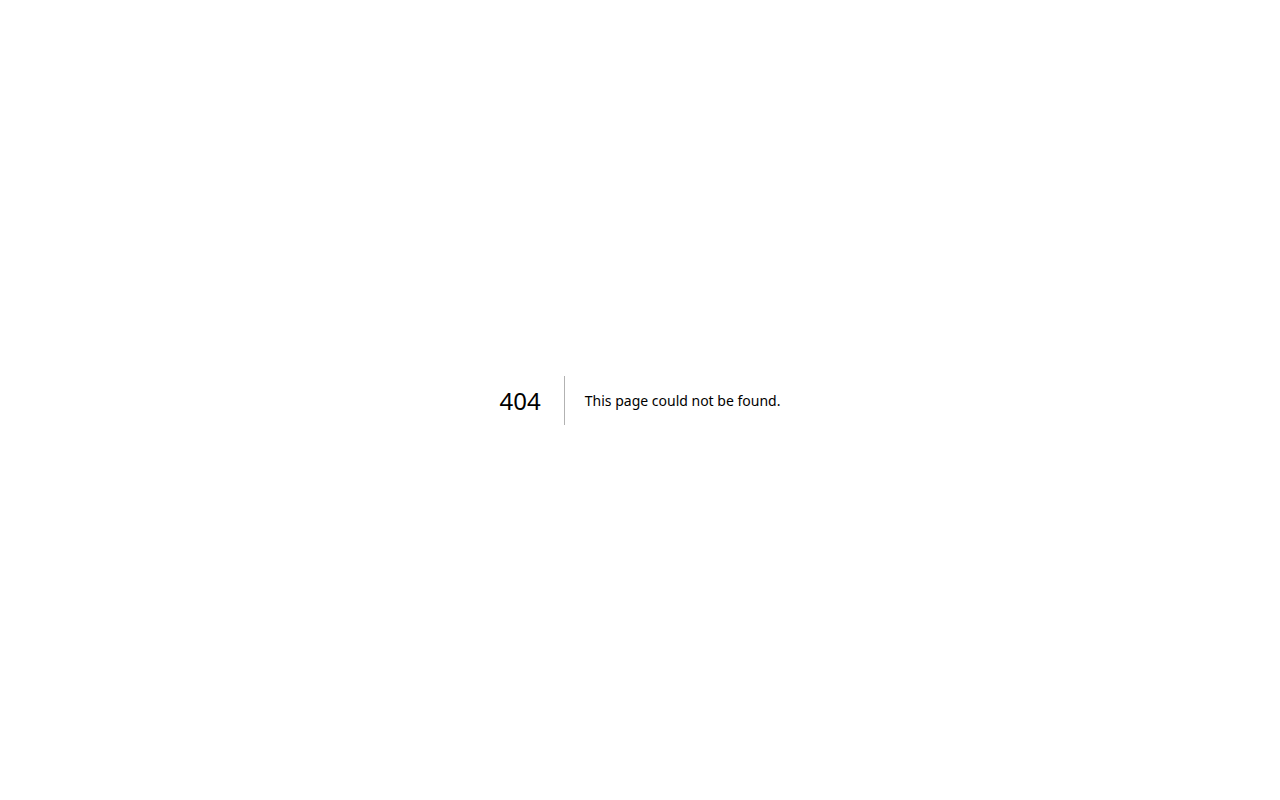
\includegraphics[width=\textwidth]{img/vet-products.png}
    \caption{Listado de productos con stock y precios}
    \label{fig:productos}
\end{figure}
